\documentclass[tikz,border=10pt]{standalone}\usepackage{tikz}\usetikzlibrary{arrows.meta,positioning}\begin{document}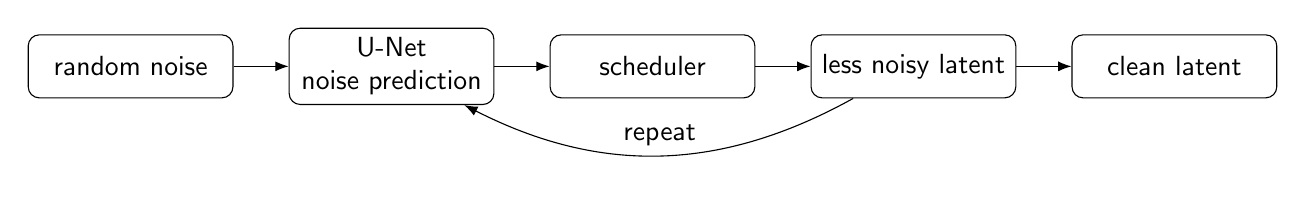
\begin{tikzpicture}[font=\sffamily,>=Latex,box/.style={draw,rounded corners,align=center,minimum width=2.6cm,minimum height=.8cm}]\node[box](a){random noise};\node[box,right=.7cm of a](b){U-Net\\noise prediction};\node[box,right=.7cm of b](c){scheduler};\node[box,right=.7cm of c](d){less noisy latent};\draw[->](a)--(b);\draw[->](b)--(c);\draw[->](c)--(d);\draw[->](d) to[bend left=28] node[above]{repeat} (b);\node[box,right=.7cm of d](e){clean latent};\draw[->](d)--(e);\end{tikzpicture}\end{document}
